\section{Introduction}
\IEEEPARstart{P}{roduction-line} integration connects process objectives, measurements, and control operations across equipment and communication interfaces. When an industrial agent proposes a setpoint change, the runtime must determine which production context and control signal the request concerns, then apply the authority and limits appropriate to that operation. The mapping depends on the production scene. For example, a cast-film line-speed setpoint may affect measured film thickness, but the setpoint and measurement are distinct process variables even when both use Message Queuing Telemetry Transport (MQTT). Command acceptance, device readback, and a later process measurement provide different evidence: acceptance records the service outcome, readback reports a returned device value, and the process measurement records what followed. Fig.~\ref{fig:control-path} illustrates this distinction.



Research on industrial agents includes service supervision and skill-based manufacturing \cite{biskupovic2025supervision,koehle2026llmdriven}. Other studies examine semantic grounding, approval, and verification for plant-facing operations, including programmable logic controller (PLC) interfaces \cite{graul2026aas,schall2026safe}. Fault-recovery planning is another area of study \cite{vyas2026detection}. These studies address different tasks and report different evidence, but they leave a systems question unresolved: how should an industrial operation boundary preserve production meaning and constrain authority when the same operation is reachable through task-mediated and direct entry paths? This paper examines that boundary without claiming a new control law or agent-reasoning algorithm.

We implement five boundary invariants: task context is descriptive and does not itself grant authority; acquisition and control mappings are direction-specific; approval is followed by route-specific revalidation; command receipts, readbacks, and later process observations remain separate; and task-mediated and direct calls converge on one guarded operation boundary. A scene binds the line, product, recipe, and run to these mappings, drivers, objectives, and limits. The contribution is integration, not a new control law or agent-reasoning algorithm. Direct API and fixture tests assess selected admission paths; a complete agent-to-device trace would require correlated harness, driver, readback, and observation records.

The contributions are:
\begin{enumerate}
  \item A production-scene configuration model that links operational context and direction-specific signal mappings to registered drivers, objectives, and limits for use at the operation boundary. (Section~III.)
  \item A task-to-device operation boundary for registered agent harnesses and direct callers that combines shared dispatch, route-specific revalidation, conditional approval, and common write guards. The reported evaluation directly exercises API, simulator, and mock-driver paths; it does not provide a complete correlated agent-to-device trace. (Sections~III--V.)
  \item An evidence-bounded evaluation of configured mappings across four simulated scenes and selected guard responses in mock-driver fixtures, supplemented by an exploratory retained-window process comparison and an injection-twin demonstration. Simulator readbacks and model-driven task outcomes are reported separately. (Section~VI.)
\end{enumerate}

\begin{figure}[!b]
\centering
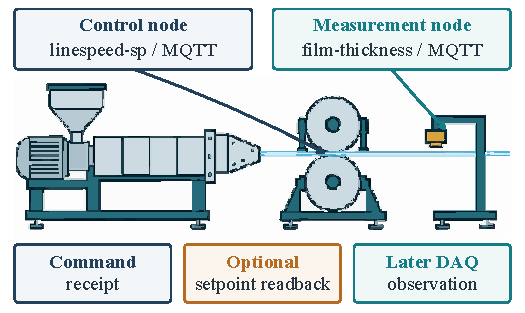
\includegraphics[width=0.98\columnwidth]{resources/fig1-vectorized-20261109.pdf}
\caption{Illustrative configured cast-film example: the line-speed setpoint and film-thickness measurement are separate nodes even though both use MQTT. Command acceptance or optional setpoint readback is distinct from the later process observation.}
\label{fig:control-path}
\end{figure}


